\chapter{Implementierung}\label{chapter_5}
 Die Implementierung hat zum Ziel die zuvor entworfenen Ansichten umzusetzen und die Realisierung der Anwendung auf der Zielplattform zu realisieren. Im Folgenden werden die Architektur und der Aufbau der Implementierung beschrieben. Anschließend werden die wichtigsten Entscheidungen, die bei der Implementierung getroffen wurden, erklärt. Die erzielten Ergebnisse werden im Anschluss präsentiert. 

\section{Anwendungsarchitektur}
Damit die Entwicklung der Anwendung beschleunigt werden kann, indem wiederverwendbare Muster in der Anwendung verwendet werden, wird zuerst eine geeignete Anwendungsarchitektur benötigt. Als erste Voraussetzung muss diese von der Zielumgebung, bzw. von der Technologie unterstützt werden. \par 

Aufgrund des Offline-Modus in der Anwendung sowie der Verwendung des Konfigurationsservers müssen zwei unterschiedliche Formen der Datenanbindung unterstützt werden. Dies hat zur Folge, dass ein einfacher Austausch der Datenanbindung in der Anwendung möglich sein muss, ohne eine Neuimplementierung der Schnittstellen auszuführen. Die Anforderung an ein ästhetisches Design kann durch eine klare Trennung der Ansicht mit den Logikkomponenten erfüllt werden. Damit ist es möglich, die Gestaltung frei von der notwendigen Logik umzusetzen und sich auf die Gestaltung der Benutzerschnittstelle zu konzentrieren. Die Architektur muss ebenfalls für Erweiterungen offen sein, damit zusätzliche Anforderungen, die beim Einsatz der Anwendung entstehen, umgesetzt werden können.

\subsection{Model-View-ViewModel}
Eine Lösung für die oben genannten Anforderungen an die Architektur bietet das von Microsoft entwickelte Model-View-ViewModel (MVVM) Entwurfsmuster. Hier wird eine strikte Trennung zwischen der Ansicht (View), der Logik (ViewModel) und den Daten (Model) vorgenommen.\par 

\begin{figure}[H]
\centering
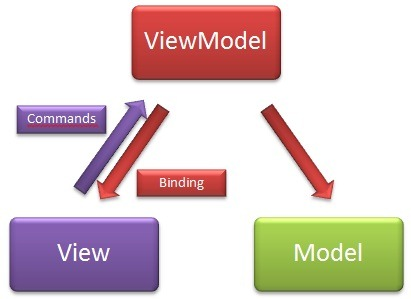
\includegraphics[height=100px]{images/mvvm}
\caption{Komponenten und Kontrollfluss im MVVM Entwurfsmuster}
\label{mvvm}
\end{figure}
Die Kommunikation der einzelnen Komponenten ist in Abbildung \ref{mvvm} dargestellt. Die unterste Ebene ist die Model-Schicht. Diese ist für das Bereitstellen und Persistieren der Daten zuständig. Es wird hierzu entweder eine Datenbank oder Webserviceschnittstelle verwendet. Wichtig bei dieser Schicht, wie in der Abbildung zu sehen, ist der unidirektionale Kontrollfluss mit dem ViewModel. Damit ist eine Manipulation der Daten nur von einer Stelle aus möglich. Dies vereinfacht das Finden von Fehlern. \par
Auf der anderen Seite ist die View. Diese Komponente ist für das Darstellen der Daten zuständig. Es werden alle Oberflächenelemente einer Benutzerschnittstelle auf dieser Ebene verwendet. Die Interaktionen des Benutzers werden auf dieser Anwendungsschicht durchgeführt. Die Auswertung der Eingaben folgt im "'Modell der Ansicht"' \cite[S.9]{bib:mvvm}, dem ViewModel. Diese Schicht ist der Vermittler zwischen den Daten und der Benutzerschnittstelle. Aus diesem Grund werden die Daten, die vom Model erhalten werden für die Ansicht aufbereitet. Die Verbindung zur View-Ebene ist dabei bidirektional, damit sowohl Benutzereingaben, als auch Veränderungen im ViewModel registriert werden. \par

Die Anforderung für einen einfachen Austausch der Datenquelle wird durch die Unabhängigkeit des Models erfüllt. Hierdurch können die Daten sowohl auf dem Gerät, als auch mit Webserviceschnittstellen geladen werden. Das MVVM Entwurfsmuster wird von der Technologie unterstützt und es sind bereits Codebeispiele vorhanden \cite{bib:winMvvm}. Mit der Trennung von View und ViewModel ist ein einfaches Erstellen von Benutzerschnittstellen möglich. Aufgrund der Unabhängigkeit beider Komponenten können diese auch separat entwickelt werden. Hierdurch wird es beispielsweise möglich, dass ein Designer und ein Programmierer unabhängig voneinander arbeiten können. Diese Vorteile sind der Grund für die Entscheidung zur Verwendung des MVVM Design Patterns anstatt des gängigen Model-View-Controlers (MVC), bei dem die View vom Controller abhängig ist und ein unabhängiges Testen der beiden Schichten nicht möglich ist.

\subsection{Anwenden des Entwurfsmusters}
Bei der Implementierung der Anwendung mussten für die Anzeige der Daten immer wiederkehrende Eigenschaften der Datensätze verwendet werden. Ein Beispiel für eine solche Eigenschaft ist der Name oder die Beschreibung eines Flugzeuges oder Upgrades. Da beim MVVM Entwurfsmuster die View nicht auf das Model zugreift, kennt es diese Datenobjekte nicht. Aus diesem Grund muss das ViewModel diese Daten konvertieren und ein neues Objekt bereitstellen. 

Ebenfalls muss bei einer Manipulation oder Auswahl der Daten die Konvertierung rückgängig gemacht werden, damit das Model die Änderungen vornehmen kann. Diese Vorgehensweise hat bei einer Veränderung der Daten zur Laufzeit Vorteile, da das ViewModel den Zeitpunkt der Persistierung entscheiden kann. Im Anwendungsbeispiel ist dies jedoch ein zusätzlicher Aufwand, der nicht benötigt wird, da keine Daten manipuliert werden, sondern eine Auswahl getätigt wird. Die eigentliche Datenbasis wird in der Anwendung nicht verändert.
Für die Vermeidung des zusätzlichen Aufwandes wurde eine neue Komponente eingeführt. Auf diese haben alle drei Ebenen im MVVM Zugriff. In dieser Komponente sind die festen Datenelemente definiert und es wird nur ein lesender Datenzugriff ermöglicht. Die konkrete Implementierung der Datensätze wird weiterhin im Model vorgenommen. Damit muss keine Konvertierung der Daten erfolgen, um der View einen Zugriff auf die Daten zu geben. \par 
\begin{figure}
\centering
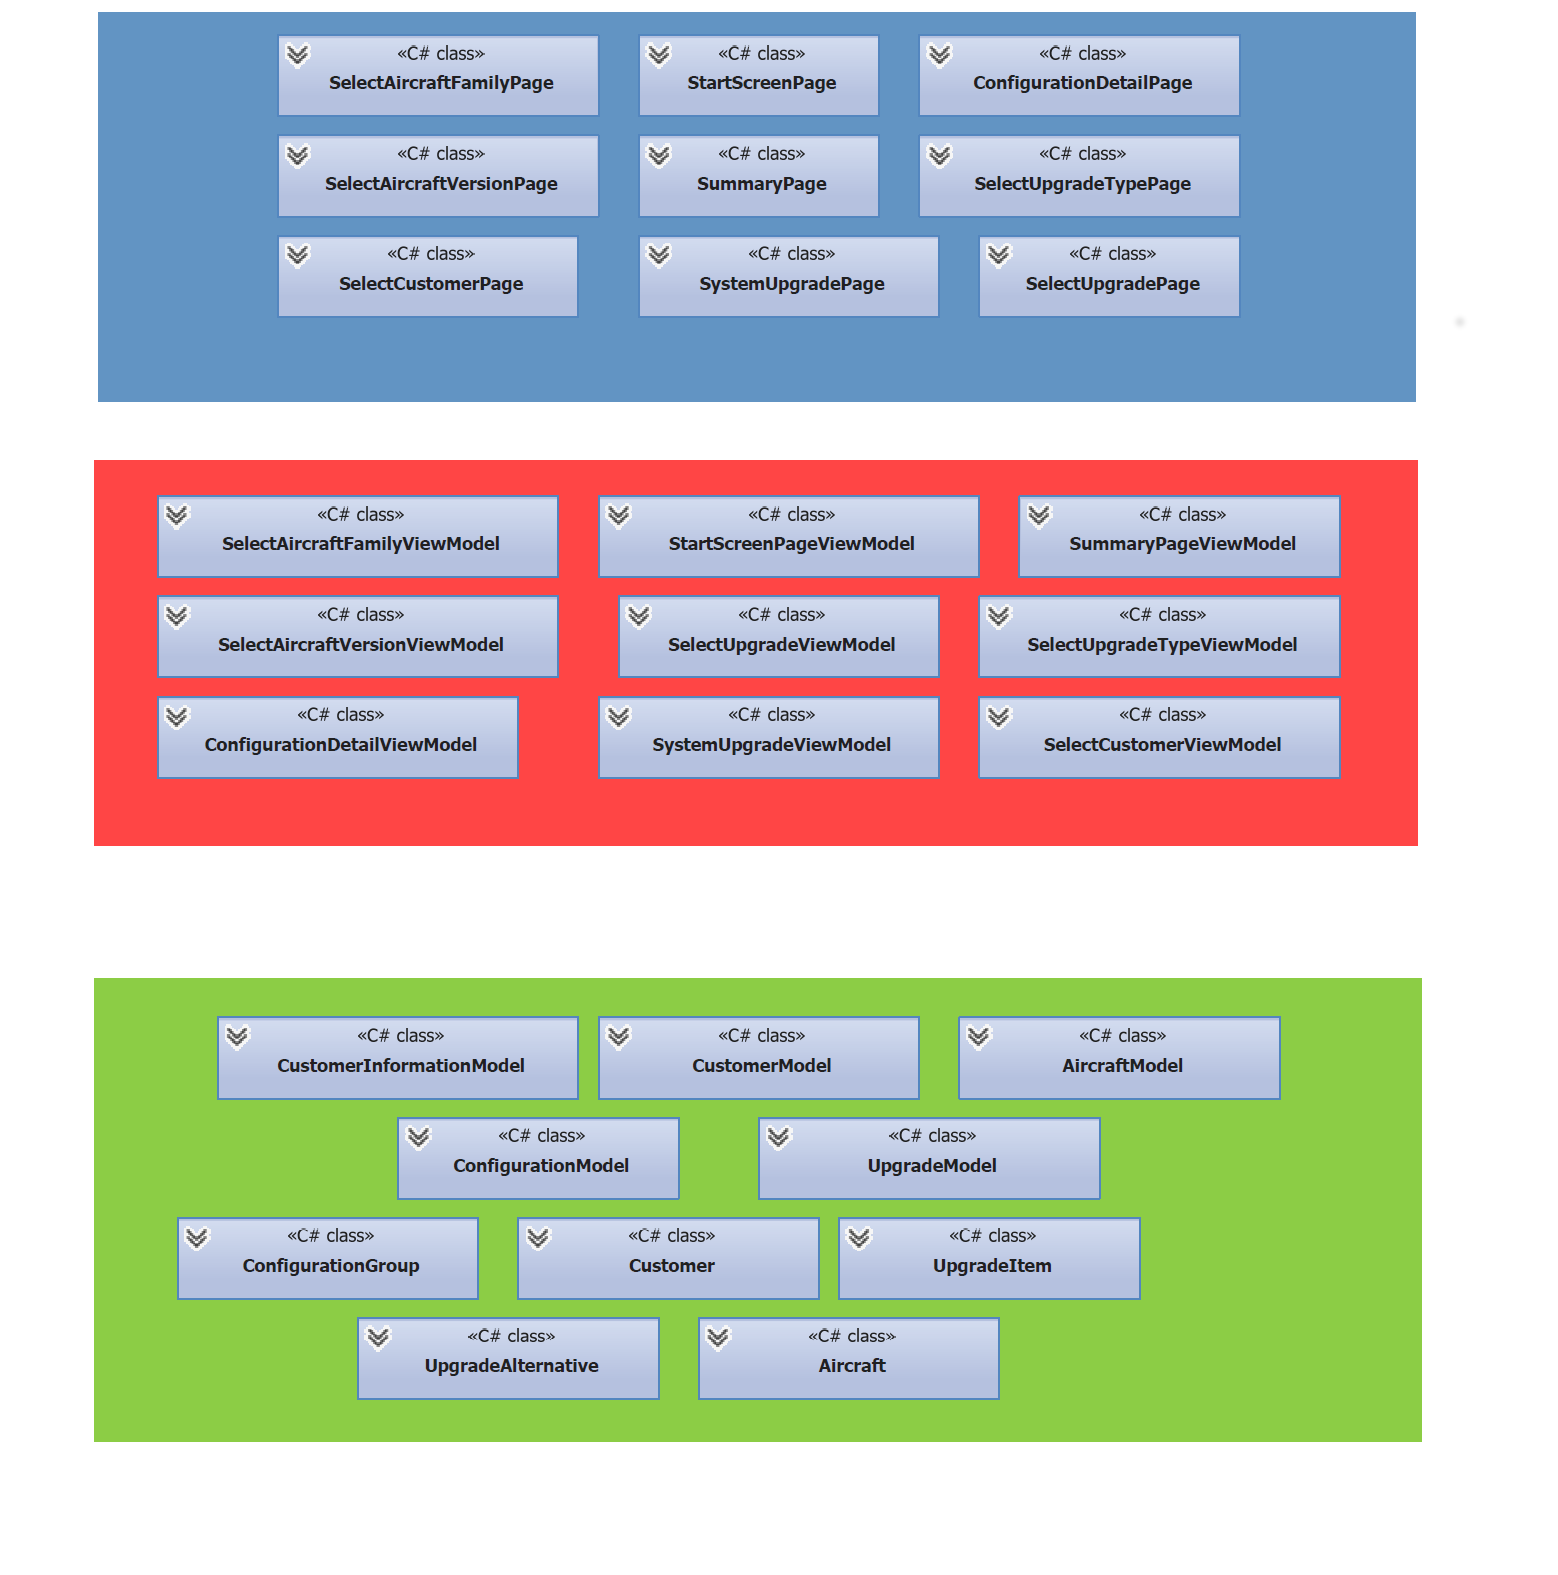
\includegraphics[width=\hsize]{images/uml_diagramm}
\caption{Klassendiagramm im MVVM Entwurfsmuster}
\label{mvvmApp}
\end{figure}
Abbildung \ref{mvvmApp} zeigt einen Ausschnitt des Klassendiagramms. Anhand der Auswahl des Upgrades, wie im Navigationsverlauf (siehe \ref{appNavigation}) zu sehen, wird die Anwendung des MVVM Entwurfsmusters demonstriert. Es werden hierfür die drei Ansichten SelectUpgradeTypePage, SystemUpgradePage und SelectUpgradePage benötigt. Alle drei erben von der Klasse Page, welche die vom Framework bereitgestellte Oberflächenklasse ist und für eine Seite der Anwendung steht. Die Definition der Page und der enthaltenen Oberflächenelemente erfolgt in sogenanntem XAML Code. Dieser ist eine XML-basierte Sprache für das deklarative Erstellen von Benutzerschnittstellen. Alle diese Komponenten lassen sich in die View-Schicht einordnen. \par 

Zu jeder Ansicht existiert ein passendes ViewModel. Damit eine bidirektionale Verbindung zustande kommt, wird für die Kommunikation von der View zum ViewModel sogenannte Bindings verwendet. Ein solches Binding bindet ein Oberflächenelement an das passende Datenelement im ViewModel. Im Beispiel ist das Grid Oberflächenelement an ein Array im ViewModel gebunden. Die Kommunikation in die entgegengesetzte Richtung erfolgt mit Events. Bei einer Änderung der Daten im ViewModel wird ein sogenanntes PropertyChangedEvent ausgeführt. Nachdem die View das Event erhalten hat, werden die Daten in der Ansicht aktualisiert. \par

Für die drei ViewModel Klassen existiert eine gemeinsame Model Klasse. Da die Daten voneinander abhängig sind, ist eine gemeinsame Verwendung sinnvoll. Das Model stellt für jedes ViewModel die passenden Schnittstellen bereit. Die Datenobjekte UpgradeType, SystemUpgrade und Upgrade sind in der Model Schicht vorhanden und werden als Datenbasis verwendet. Die bereitgestellten Methoden verwenden Objekte dieser Klassen. Damit die Datenobjekte auch in der View verwendet werden können, ist die Definition als Interface in die DataCommon Komponente ausgelagert. Diese kann von allen drei Schichten der Anwendung verwendet werden. Im Beispiel wird die Verwendung in den ViewModel Klassen demonstriert. Hier werden die Datenelemente, die für das Binding mit der View benötigt werden als ein Array des Interface bereitgestellt. Dies sorgt für eine einheitliche Kommunikation der drei Ebenen und vermeidet eine Konvertierung der Daten im ViewModel.


\section{Navigation}
Eine besondere Herausforderung bei der Implementierung ist die Navigation. Diese muss zuerst in das Entwurfsmuster eingeordnet werden. Es muss entschieden werden, in welcher Ebene navigiert wird. Der Wechsel der Ansichten ist eine Aufgabe der View. Diese bestimmt, wie zu einer neuen Seite navigiert wird. In dieser Ebene werden auch die konkreten Navigationsmethoden angeboten. Andererseits ist die Entscheidung darüber, wann in welche Ansicht gewechselt wird eine Angelegenheit des ViewModels. Diese wertet die Auswahl eines Klicks aus und ist damit für dessen Bearbeitung zuständig. Weiterhin werden Objekte zwischen den beiden ViewModels ausgetauscht. Aus diesem Grund muss es eine Möglichkeit für den Austausch geben. \par 

Die Lösung des Problems erfolgt mit dem Ansatz der Inversion of Control \cite{bib:ioc}. Bei diesem Prinzip geht es um die Auflösung von Abhängigkeiten. Anstatt ein Objekt direkt zu erzeugen, wird es von einer zentralen Stelle verwendet. Die Abhängigkeit wird damit von außerhalb des aktuellen Codes hinzugefügt. Dieser Ansatz hat besonders bei Softwaretests große Vorteile, da andere Objekte für Testzwecke verwendet werden können.  \par
\begin{figure}[H]
\centering
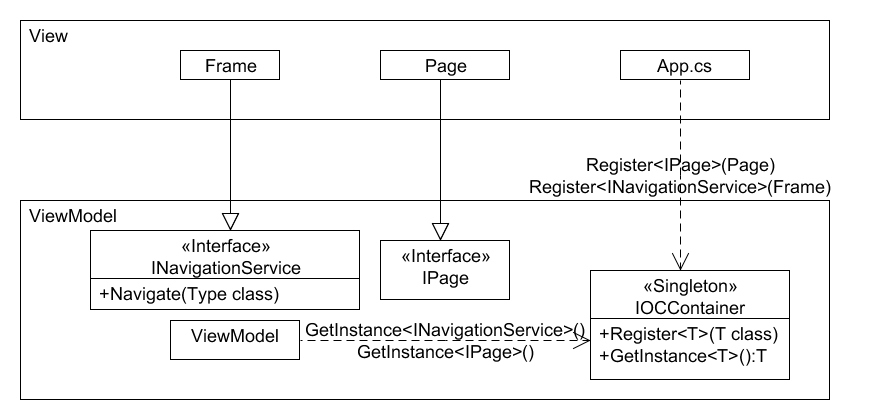
\includegraphics[width=\hsize]{images/dependencyInjection}
\caption{Navigation mit Inversion of Control}
\label{ioc}
\end{figure}
Die Umsetzung des Prinzips ist in Abbildung \ref{ioc} dargestellt. Damit eine Verwendung der einzelnen Klassen aus der View im ViewModel möglich ist, wird für jede Ansicht (Page) ein passendes Interface (IPage) definiert. Eine Navigation wird beim Windows 8 Framework mit der Frame Klasse durchgeführt. Dieses implementiert das INavigationService Interface, welches zwei Navigationsmethoden beinhaltet. Eine Methode kann mit einem Parameter für das neue ViewModel ausgeführt werden, die Andere ohne Parameter. Beim Start der App Klasse werden die einzelnen Pages und der Navigationsframe mit den definierten Interfaces im IOCContainer registriert. Der Container befindet auf der ViewModel  Ebene. Für eine Navigation werden die Zielpage und der Navigationsservice mit der GetInstance<T> Methode erhalten. Anschließend kann die passende Navigationsmethode entweder mit oder ohne Parameter ausgeführt werden. \par 
\begin{figure}
\begin{lstlisting}
private void SaveSelectionAndNavigateToSummaryPage(DataCommon data)
{
       var selectedProgramm = GetSelectedProgramm(data.UniqueId);
       _model.SelectAircraftProgramm(selectedProgramm);
       var classToNavigate = SimpleIoc.Default.GetInstance<ISummary>();
       var navigationService = SimpleIoc.Default.GetInstance<INavigationService>();
       navigationService.Navigate(classToNavigate.GetType());
}
\end{lstlisting}
\caption{Auszug des AircraftFamilyViewModels (siehe Anhang A)}
\label{navigateMethod}
\end{figure}

In Codebeispiel \ref{navigateMethod} wird ein solcher Navigationsvorgang im ViewModel demonstriert. Dieser Auszug ist aus der Flugzeugpgrogramm Auswahl entnommen. Nachdem ein Programm ausgewählt wurde, wird zuerst die Auswahl im Model gespeichert. Im zweiten Schritt erhält man die  Zusammenfassungsseite mit dem Interface (ISummary) vom Container. Die Navigation erfolgt anschließend mit dem Navigationsservice.
\par
Mit diesem Ansatz gelingt es, die Darstellung und die Entscheidung, welche Ansicht bei welchem Inhalt verwendet wird, der View Schicht zu überlassen. Der Wechsel von Ansichten wird mit Methoden durchgeführt, die eine Ansicht bereitstellt. Das ViewModel kann entscheiden, wann eine Navigation durchgeführt wird. Durch die Verwendung des Containers ist eine zentrale Stelle vorhanden, die jederzeit verwendet werden kann. Bei einer Navigation können Parameter übergeben werden, die eine Kommunikation der ViewModels ermöglicht. 

\section{Ergebnisse der Implementierung}
Die Entwürfe des vorigen Kapitels konnten detailreich bei der Implementierung abgebildet werden. Im Folgenden werden die wichtigsten implementierten Ansichten kurz vorgestellt.

\subsection{Startseite und Flugzeugprogrammauswahl}

Das Ergebnis für die Startseite (siehe \ref{startScreenImpl}) konnte vom Entwurf übernommen werden. Für die Anzeige des aktuellen Status der Konfiguration wurde eine Signalfarbe und ein passendes Icon hinzugefügt. Ebenfalls wurde der Text durch passende Icons ausgetauscht (vgl. \ref{startSketch}). \par
\begin{figure}
\centering
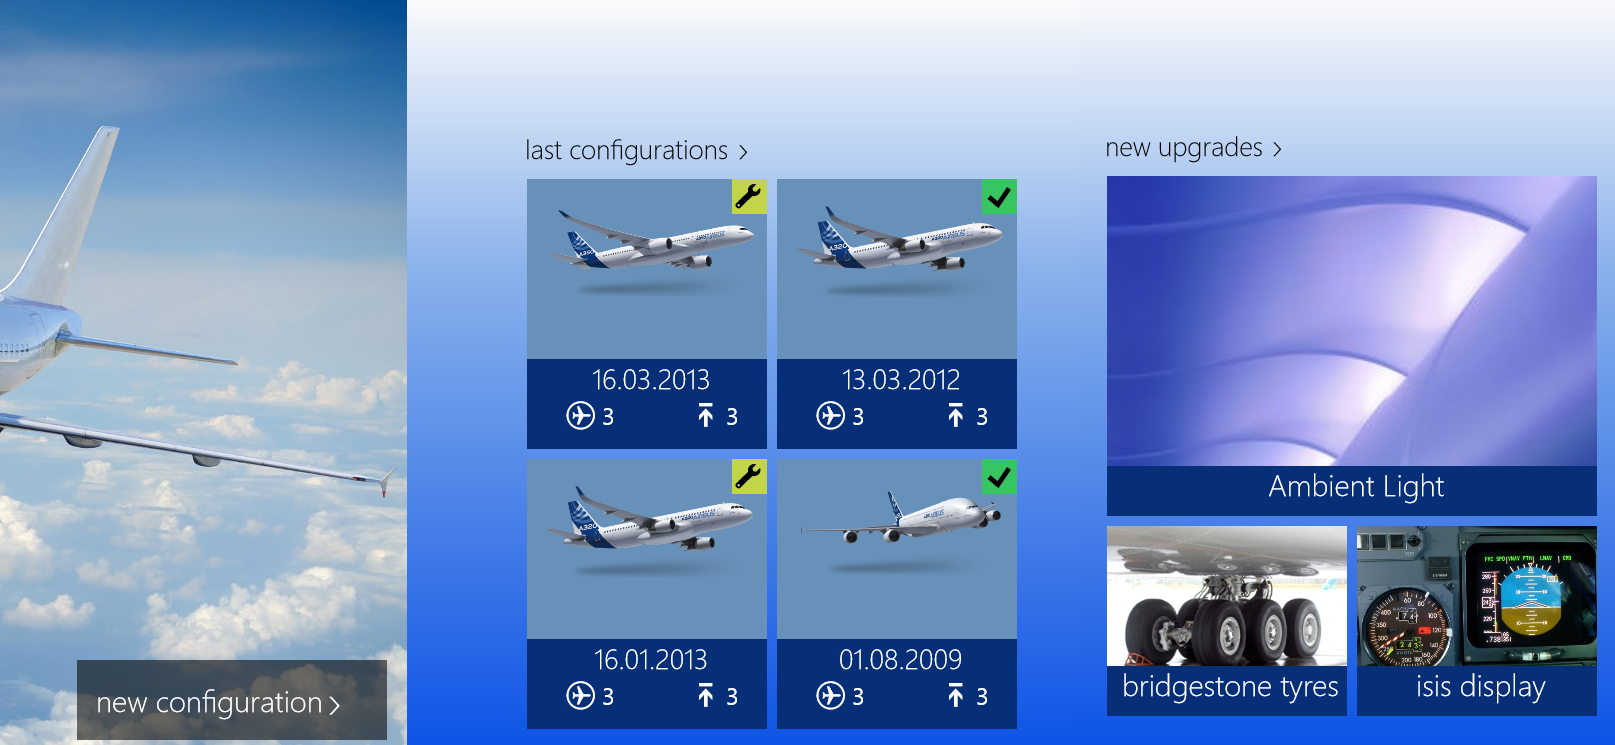
\includegraphics[width=\hsize]{images/impl/start_screen_impl}
\caption{Auszug der implementierten Startseite}
\label{startScreenImpl}
\end{figure}
Bei der Auswahl des Flugzeugprogramms (siehe \ref{aircraftProgrammImpl}), dass direkt nach dem Start einer neuen Konfiguration angezeigt wird, wurde der Begriff Familie statt Programm verwendet. Die Darstellung enthält ein zugehöriges Flugzeug  in der passenden Kachel.


\begin{figure}[H]
\centering
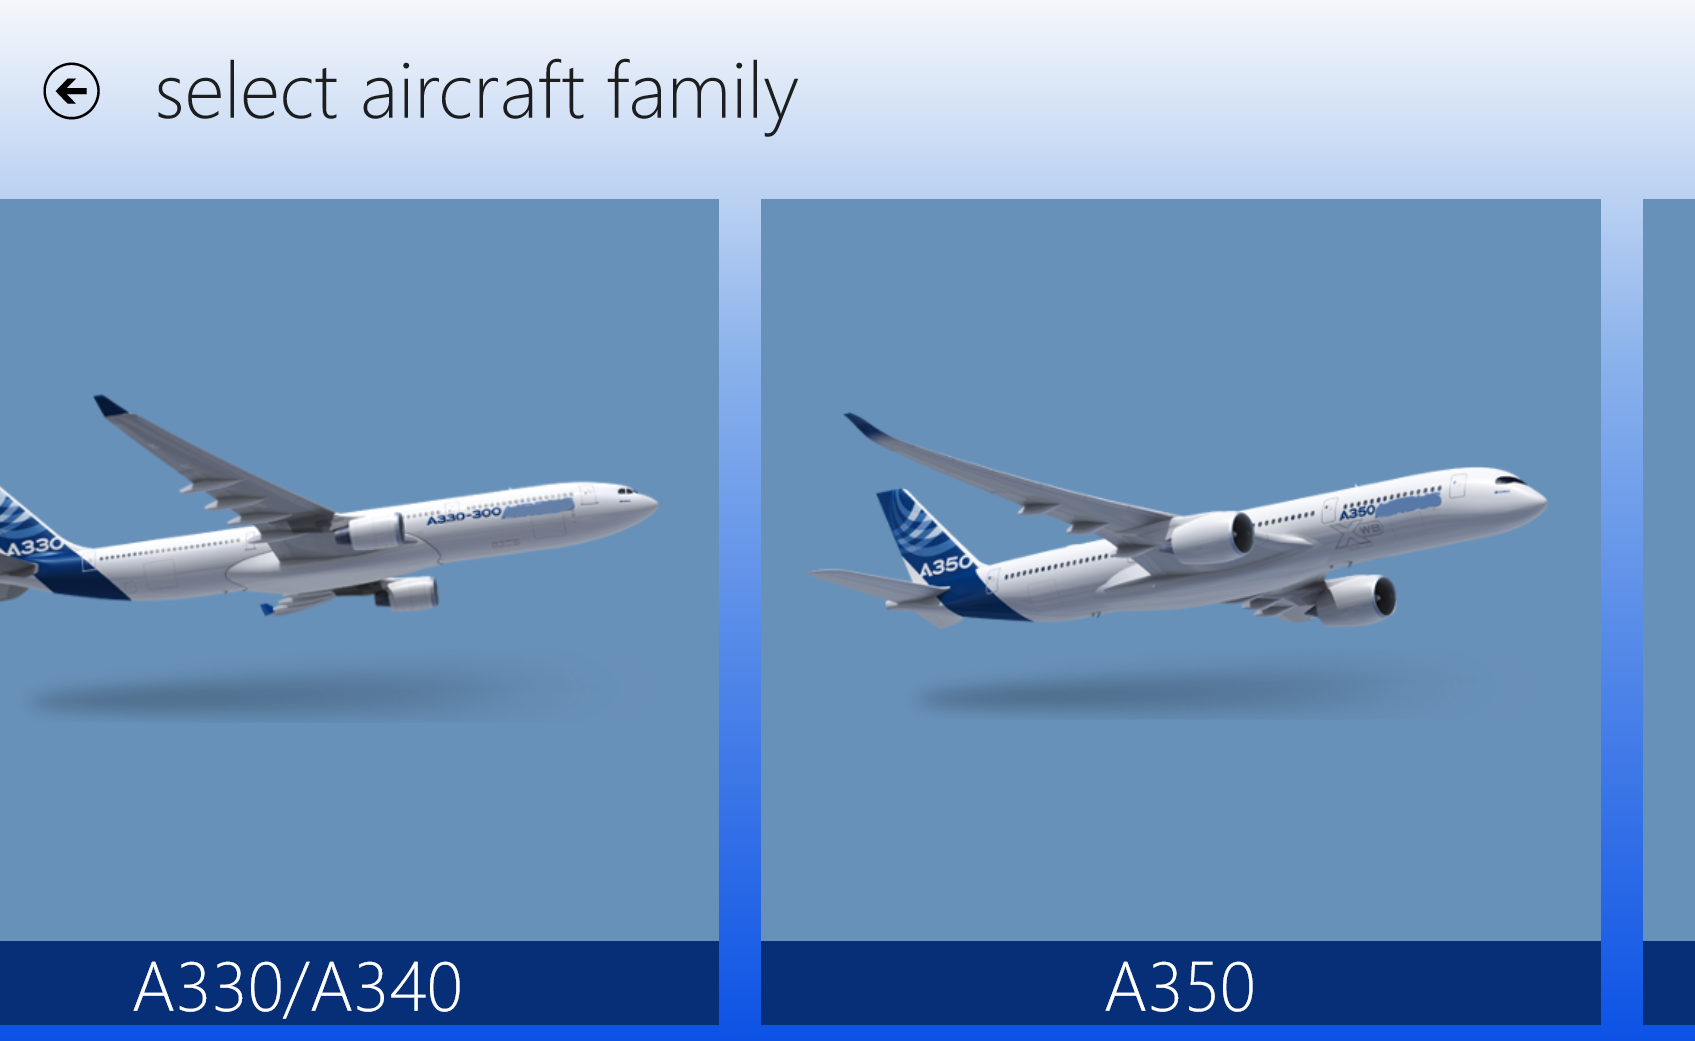
\includegraphics[width=\hsize]{images/impl/select_aircraft_family_impl}
\caption{Auszug der implementierten Flugzeugprogrammauswahl}
\label{aircraftProgrammImpl}
\end{figure}

\subsection{Upgradeauswahl}
\begin{figure}[H]
\centering
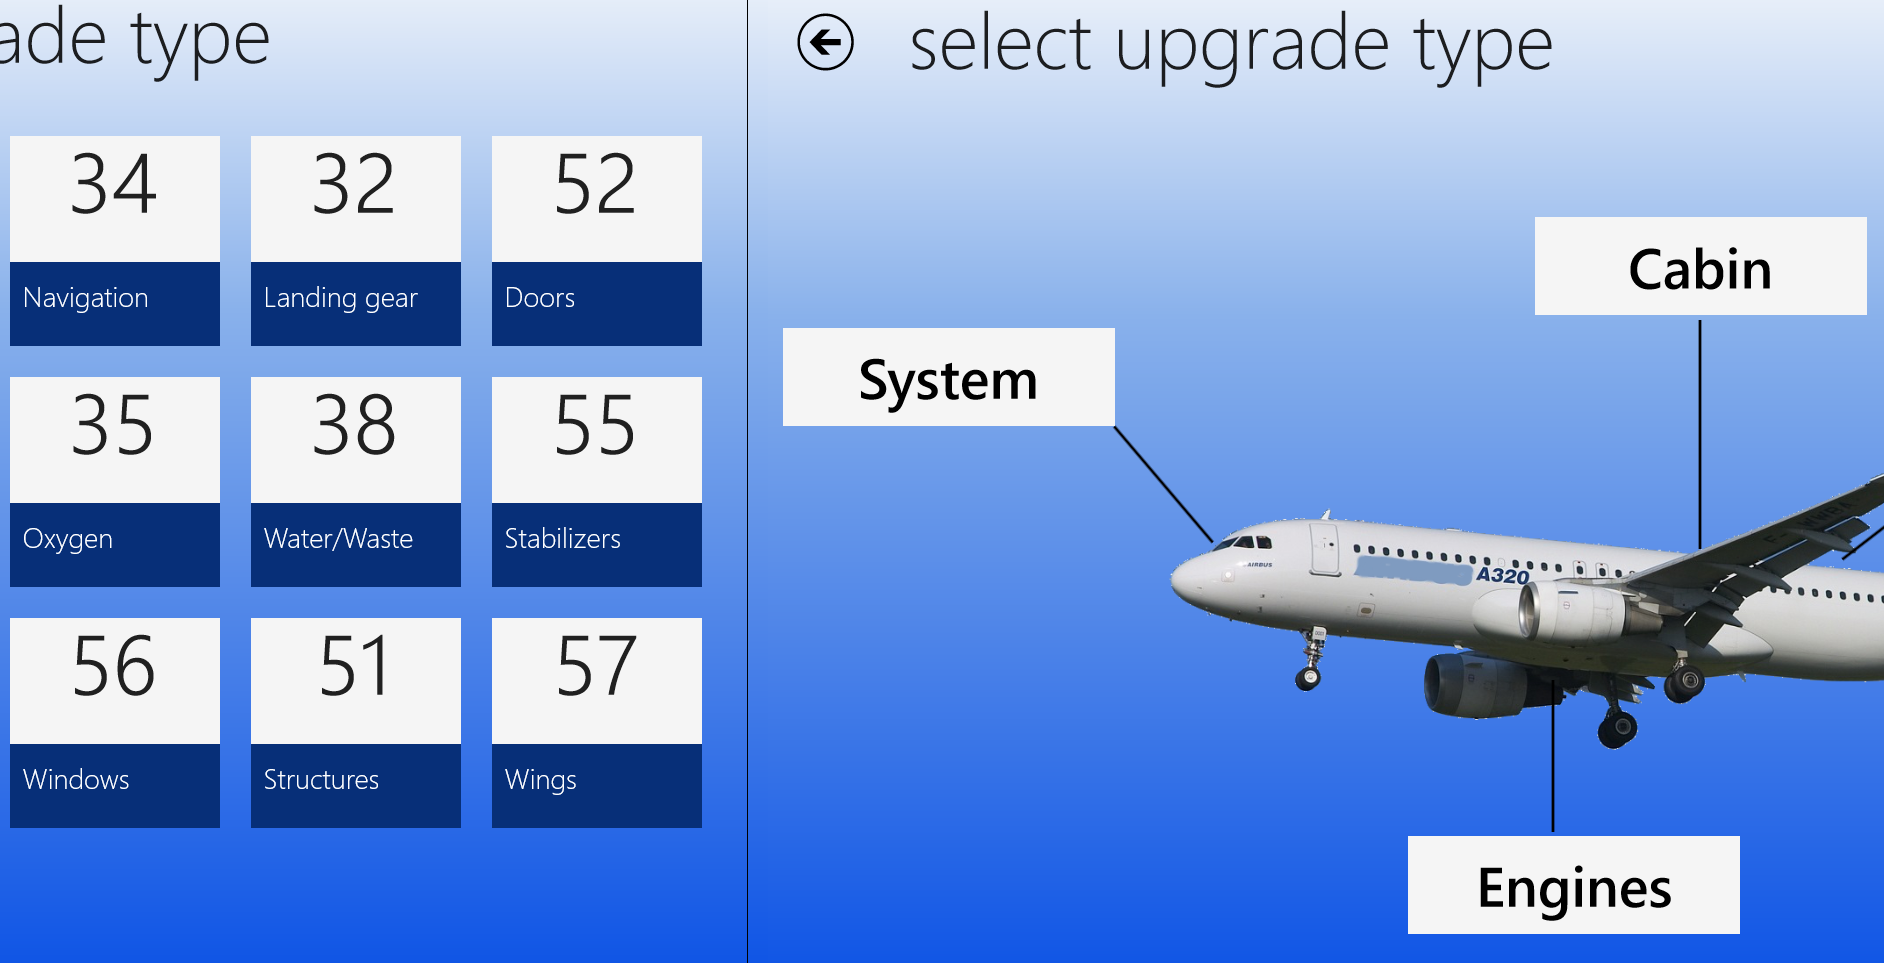
\includegraphics[width=\hsize]{images/impl/select_upgrade_type_impl}
\caption{Auszug der implementierten Upgradetypauswahl}
\label{upgradeTypeSelectionImpl}
\end{figure}
In Abbildung \ref{upgradeTypeSelectionImpl} ist die Auswahl des Upgrade Typs zu sehen. Diese wurde mit der FlipView (vgl. \ref{flip}) umgesetzt. Beim Aufruf der Seite ist die Upgradetyp Auswahl (rechtes Bild) zu sehen.  Um in den Expertenmodus (linke Seite) zu kommen, wird eine Wisch-Geste nach von links nach rechts durchgeführt. Dieses "'flippen"' unterstützt den Experten bei einer schnelleren Navigation.


Bei der Auswahl der Upgrades, wie in Abbildung \ref{upgradeSelectionImpl} zu sehen, sind viele Informationen auf der Ansicht enthalten. Auf der rechten Seite können die einzelnen Unterkategorien ausgewählt werden. Die Details zu der Auswahl erscheinen auf dem rechten Bildschirmrand. Die einzelnen Upgrades werden auf das Wesentliche reduziert. Nach der erfolgten Auswahl wird die derzeitige Selektion auf der unteren AppBar angezeigt. Ein Abschluss der Auswahl sowie die Navigation in die Zusammenfassungsseite erfolgt mit Hilfe eines Button. \par 
\begin{figure}[H]
\centering
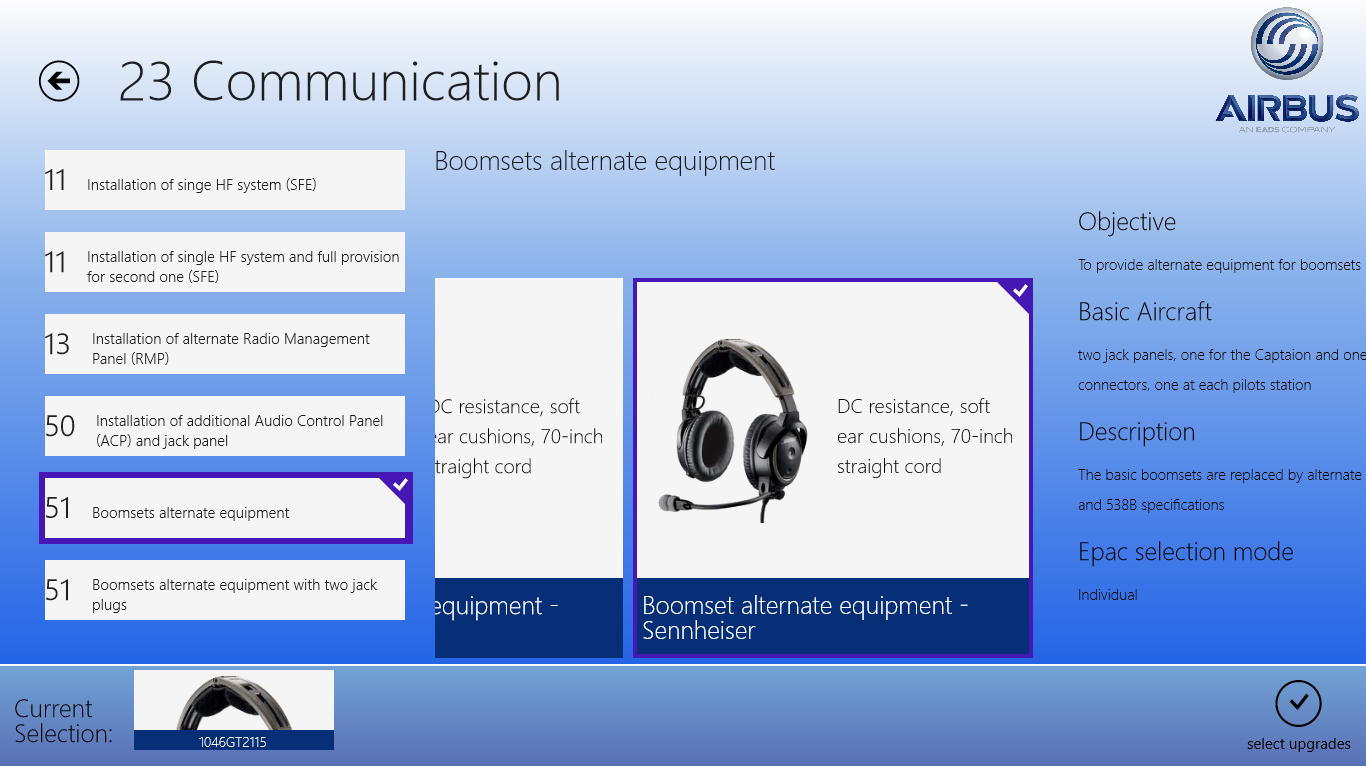
\includegraphics[width=\hsize]{images/impl/select_upgrade_impl}
\caption{Auszug der implementierten Upgradeauswahl}
\label{upgradeSelectionImpl}
\end{figure}

\subsection{Flugzeugauswahl}
Die Auswahl der Flugzeuge (siehe \ref{aircraftSelectionImpl}) ist mit den Kacheln im Grid umgesetzt worden. Für eine schnelle Auswahl von großen Datensätzen wurde der semantische Zoom in dieser Ansicht verwendet. Damit dem Benutzer mehr Möglichkeiten gegeben werden, kann er die Gruppierung der Flugzeuge mit eine Auswahlliste selbst festlegen. Abbildung \ref{aircraftSelectionZoomImpl} zeigt den semantischen Zoom mit den verschiedenen Flugzeugtypen gruppiert.  In dieser Ansicht wird die Anzahl der Elemente in der Gruppe angezeigt. 
\begin{figure}[H]
\centering
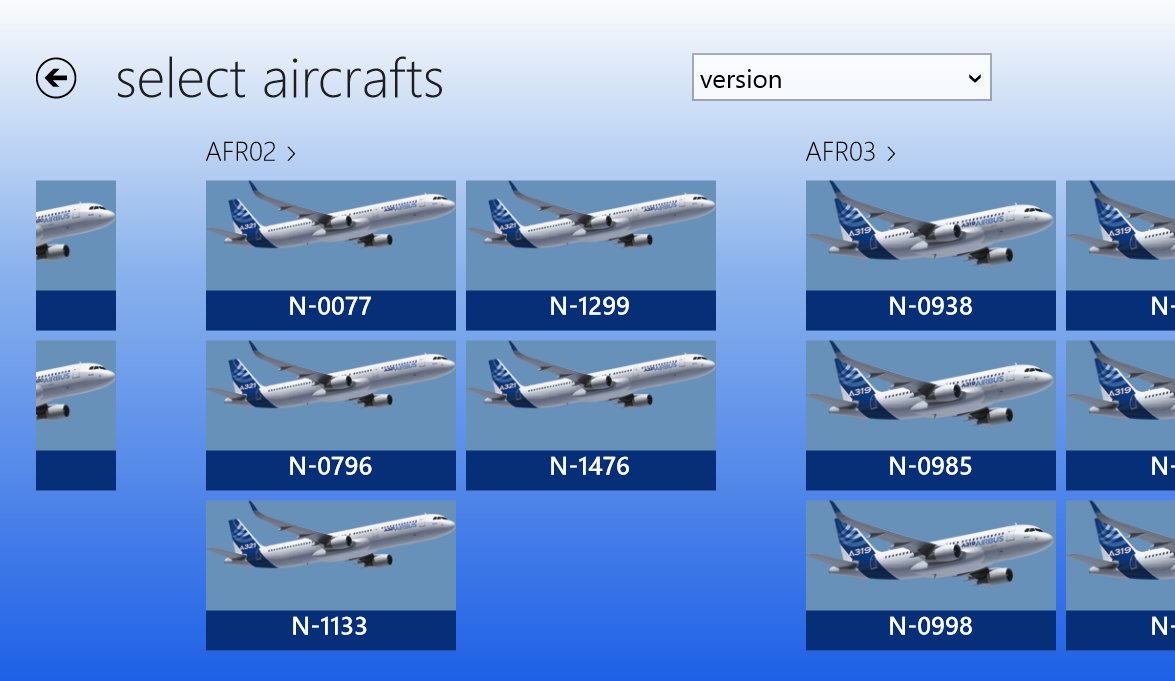
\includegraphics[width=400px]{images/impl/select_aircrafts_impl}
\caption{Auszug der implementierten Flugzeugauswahl}
\label{aircraftSelectionImpl}
\end{figure}
\begin{figure}[H]
\centering
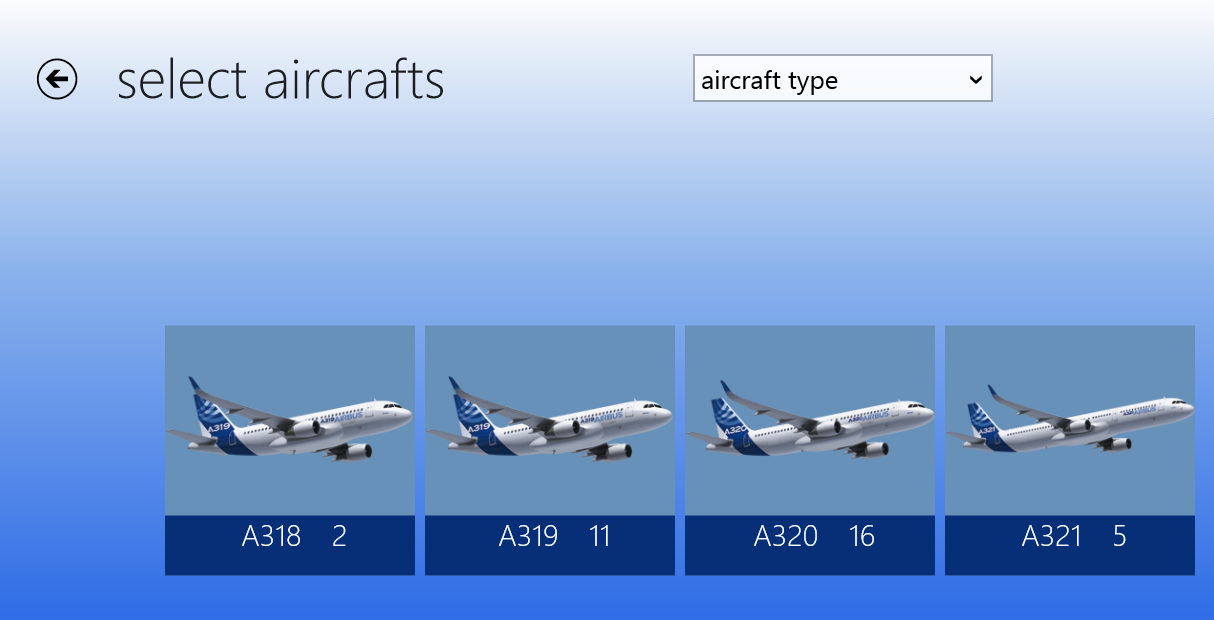
\includegraphics[width=400px]{images/impl/semantic_zoom_impl}
\caption{Herausgezoomte Ansicht der Flugzeugauswahl}
\label{aircraftSelectionZoomImpl}
\end{figure}

\subsection{Konfigurationsansicht}
Eine Übersicht der Konfigurationsergebnisse wird in der Zusammenfassungsseite (siehe \ref{configurationResultImpl}) gezeigt. Im Screenshot sind zwei Konfigurationsgruppen angezeigt, die beide komplett sind und somit auch bestellt werden können. Der Abschluss der Konfiguration erfolgt mit den Buttons in der unteren AppBar. Die obere Leiste zeigt die Navigationsmöglichkeiten, die in der kompletten Anwendung vorhanden sind. Auf der rechten Seite können die Hauptansichten ausgewählt werden und auf der linken Seite kann zur Startseite navigiert werden. \par 
\begin{figure}[H]
\centering
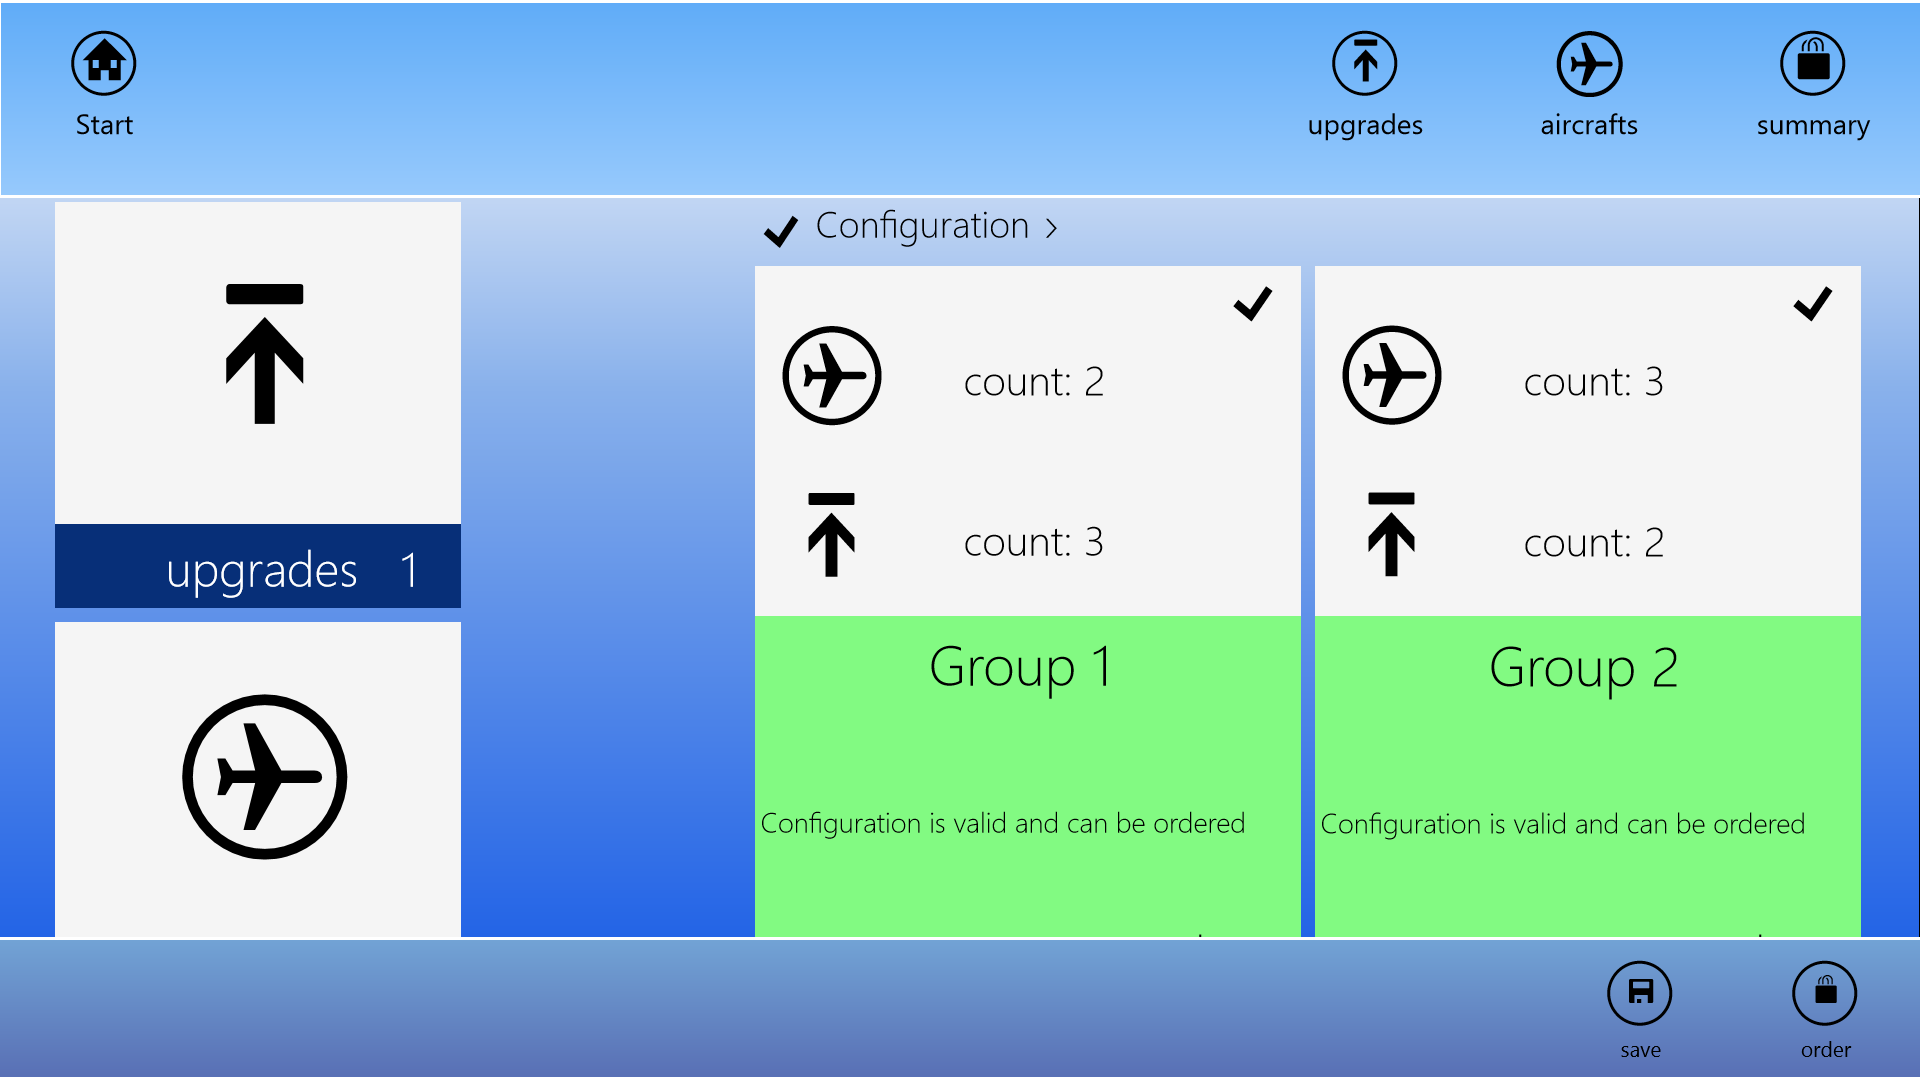
\includegraphics[width=\hsize]{images/impl/app_bar_impl}
\caption{Konfigurationsgruppen und Navigationsbar in der Zusammenfassung}
\label{configurationResultImpl}
\end{figure}
Die Auswahl der Alternativen ist in Abbildung \ref{alternativeSelectionImpl} dargestellt. Hier werden zuerst die möglichen Alternativen angezeigt, die ausgewählt werden können. Zusätzlich sind die zuvor ausgewählten Upgrades vorhanden sowie die zur Konfigurationsgruppe gehörigen Flugzeuge. 
\begin{figure}[H]
\centering
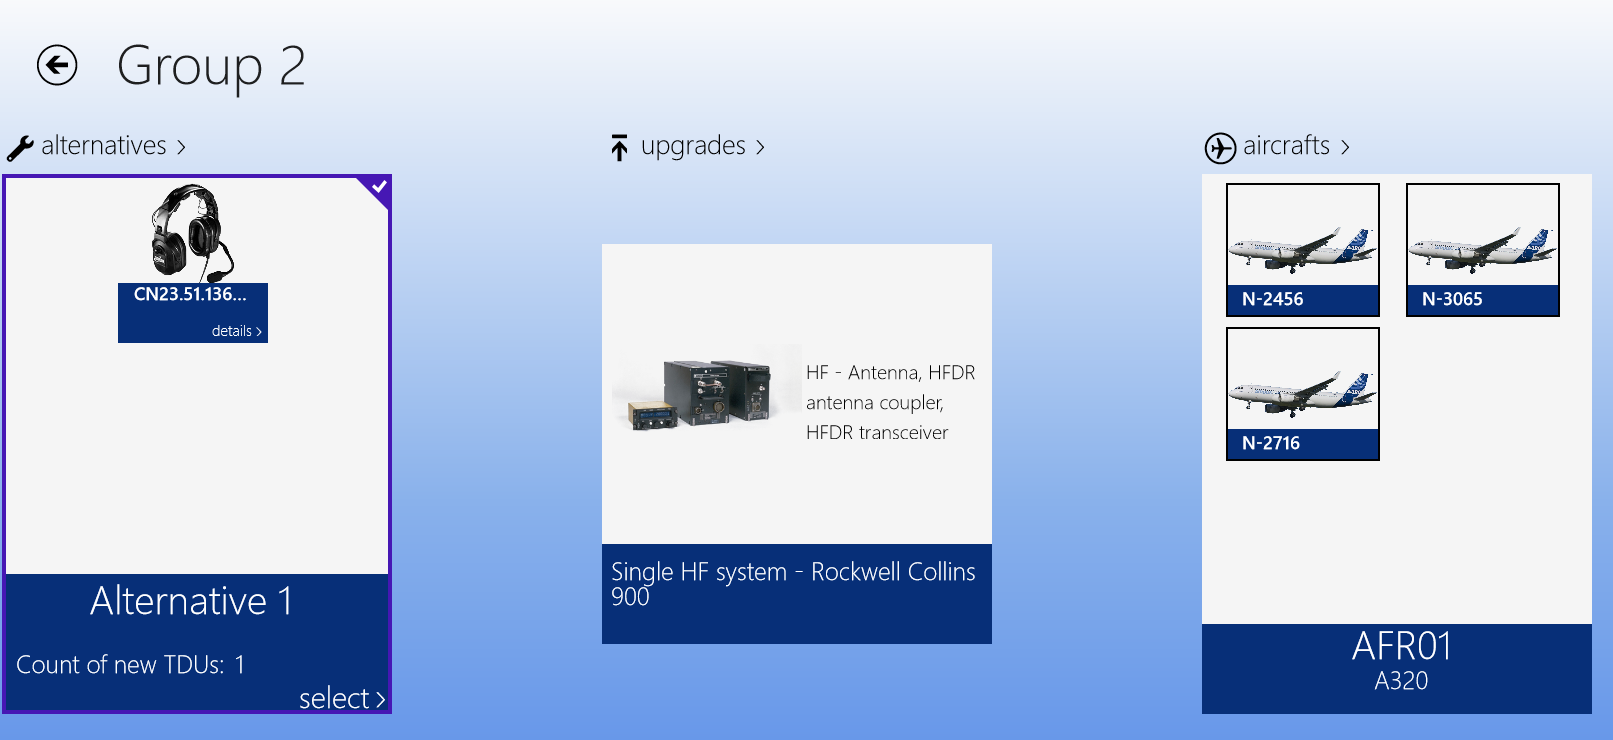
\includegraphics[width=\hsize]{images/impl/alternative_impl}
\caption{Alternativenauswahl für die zweite Konfigurationsgruppe}
\label{alternativeSelectionImpl}
\end{figure}

 